\documentclass{article}
\usepackage{graphicx}
\usepackage{longtable}
\usepackage{hyperref}
\usepackage{array}
\usepackage{multicol}
\usepackage[table]{xcolor}

\title{Meal Plan Generator}
\author{SEDEV210 - Programming for Data Science\\Masters of Science in Data Science}
\date{}

\begin{document}

\maketitle



\subsection*{LT6 Members}
\begin{multicols}{2}
\begin{itemize}
    \item Cayco, Francis Mark M.
    \item Pelayo, Angela Elaine F.
    \item Sangalang, Luisito II M.
    \item Madarang, Andrea Yna M.
    \item Verma, Srijat
\end{itemize}
\end{multicols}

\tableofcontents

\section{Rationale}
Meal Plans have increased in popularity over the past years. The benefits of which is the reduced mental load in deciding and planning meals which will free up time and make it easier for consumers to be able to meet their health or fitness goals. Meal plans offer targeted diets that would assist consumers in ensuring that they are aligned to their targets, may it be to reduce weight, to gain muscle, or to improve their overall health with a well-rounded meal.

The proposed system will take in the information that the users will provide regarding their biodata and their targets to determine which plan would best suit them. It will provide recommendations on the types of foods that they should focus on to be able to meet their desired goals.

\subsection{Data Requirements}
The biodata required would be the biological gender of the consumer, age, fitness level, current weight, and target weight. These questions will be prompted at the beginning of their application to provide the information needed to perform the prediction proposed. The data will also require a person’s current activity level to be able to account for the daily requirements of each individual.

\subsection{Food Mapping}
Food information is stored within the program that contains information regarding the types of food and their caloric impact/portion size. The program will cross-reference the types of food with the needs of the user to build the meal plan provided for the selected duration.

\subsection{Algorithm-Based Meal Planning}
By using the biodata provided, the system will be able to calculate the optimal meal plan for the customer. Taking into consideration the person’s current activity level and their goals, the system will be able to account for the number of calories each individual needs to either maintain a calorie deficit or support an increase in muscle gain.

\section{Features}
\subsection{Product Flow Diagram}
\begin{figure}[!ht]
\begin{center}
  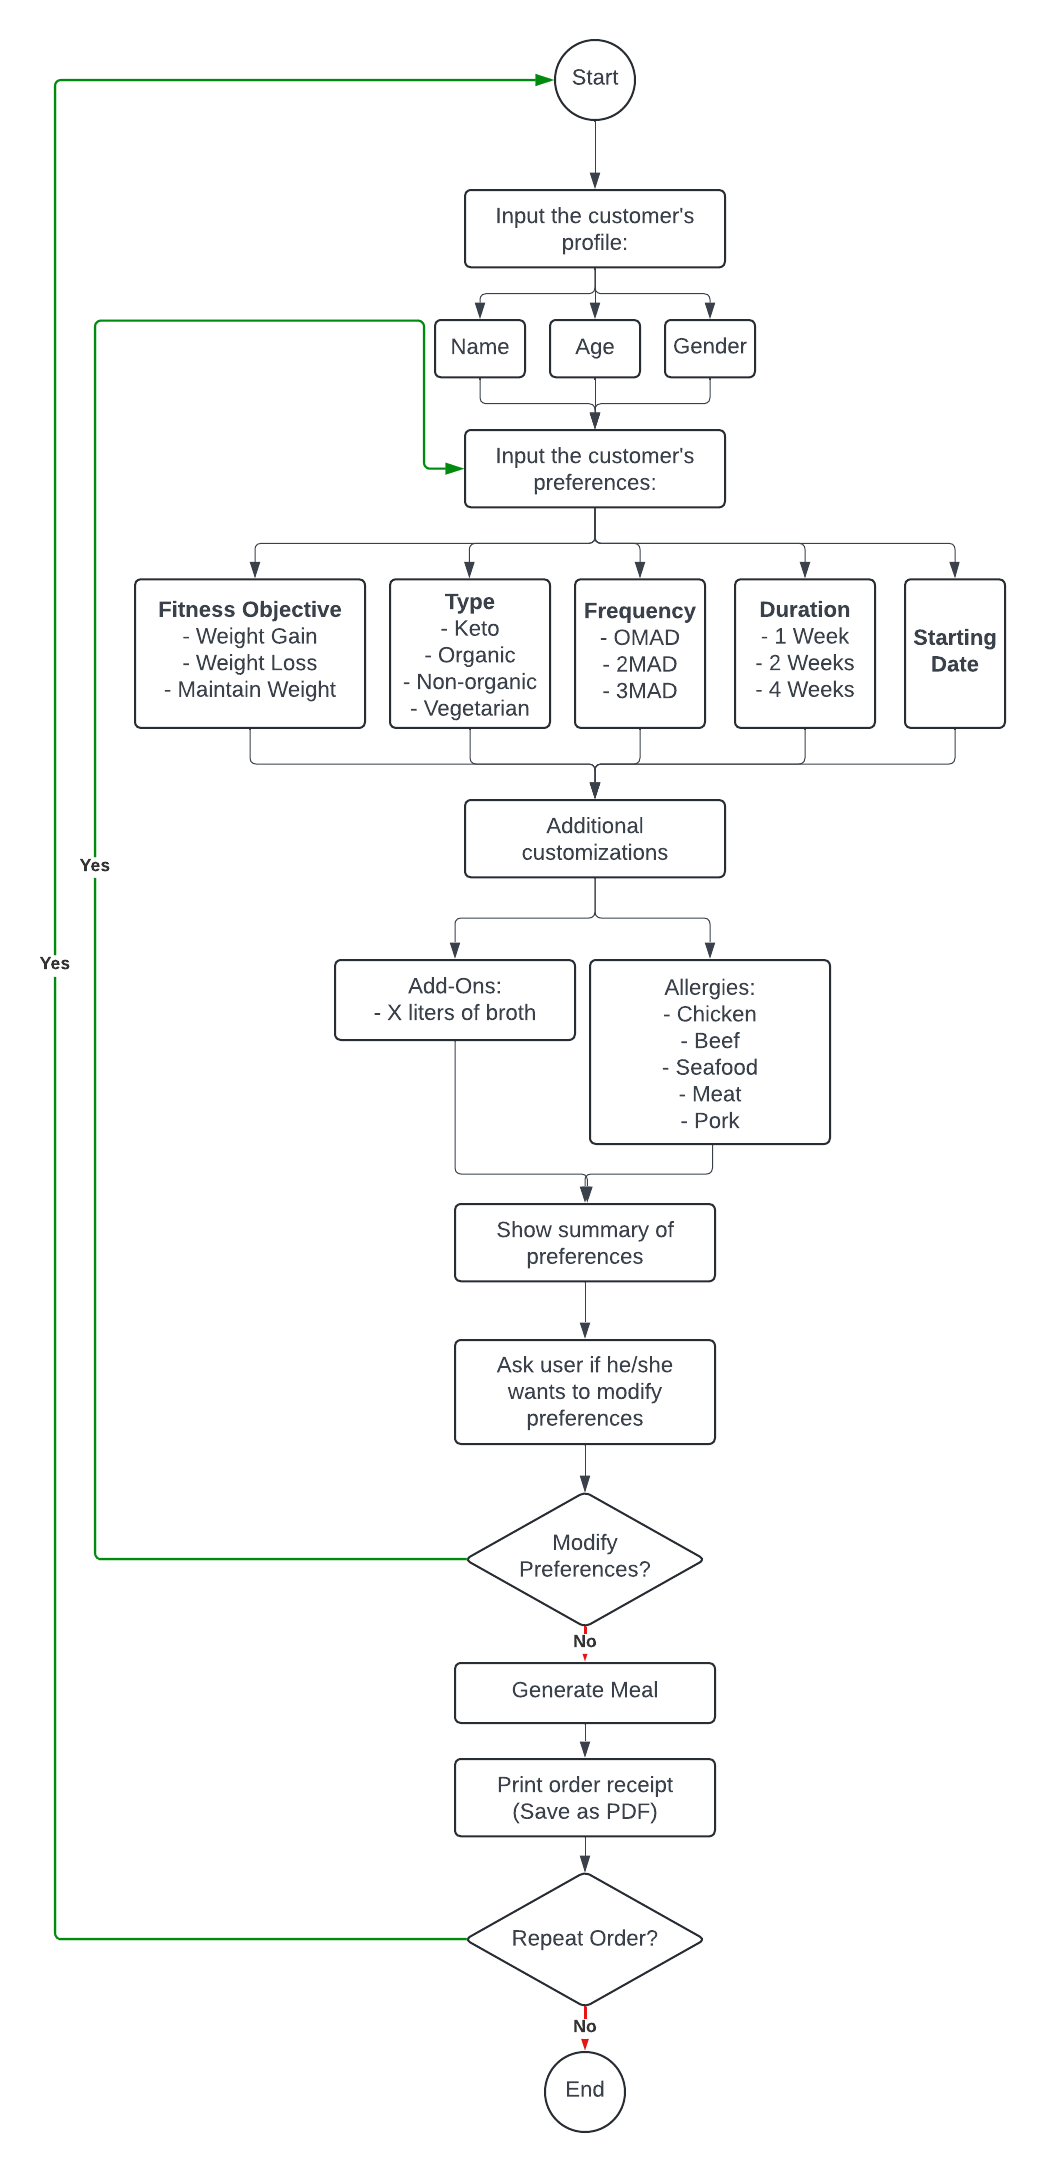
\includegraphics[width=0.6\textwidth]{docs/meal_planner_flowchart.png}
  \caption{Product Flow Diagram}
\end{center}
\end{figure}
The process begins with the user inputting the customer's profile, which includes the customer's name, age, and gender. After capturing these details, the user proceeds to input the customer's preferences. These preferences cover various aspects such as the customer's fitness objective, where options include:

\begin{itemize}
    \item Weight Gain
    \item Weight Loss
    \item Maintain Weight
\end{itemize}

Next, the user selects the type of diet, with options like:

\begin{itemize}
    \item Keto
    \item Organic
    \item Non-organic
    \item Vegetarian
\end{itemize}

The frequency of meals is then chosen, offering the customer the choice between:

\begin{itemize}
    \item OMAD (One Meal a Day)
    \item 2MAD (Two Meals a Day)
    \item 3MAD (Three Meals a Day)
\end{itemize}

Following this, the user sets the duration of the meal plan, which can be:

\begin{itemize}
    \item 1 Week
    \item 2 Weeks
    \item 4 Weeks
\end{itemize}

and specifies the starting date for the plan.

Additionally, the user can customize the meal plan further by adding specific preferences like the amount of broth or indicating any allergies (such as chicken, beef, seafood, meat, or pork). Once all preferences are entered, a summary of these preferences is shown. The user is then asked if they would like to modify any of the preferences. If modifications are needed, the user is taken back to the preferences input step.

If no modifications are needed, the process continues with generating the meal plan. The user then has the option to print the order receipt and save it as a PDF. Finally, the user is asked if they would like to repeat the order. If they choose to repeat, the process starts over; if not, the process ends.



\subsection{Meal Criteria}
\subsubsection{Keto Meals}
\begin{itemize}
    \item Low-carb, high-fat diet preference
    \item Aiming for weight loss, blood sugar management, or cognitive benefits
    \item Interested in keeping carbohydrate intake at or below 5-10\% of total daily intake
\end{itemize}

\subsubsection{Organic Meals}
\begin{itemize}
    \item Prioritizes consumption of ingredients without synthetic pesticides, herbicides, or GMOs
    \item Prefers sustainably sourced, environmentally friendly foods
    \item Concerned about the purity and quality of food, avoiding synthetic additives
\end{itemize}

\subsubsection{Non-Organic Meals}
\begin{itemize}
    \item Budget-conscious, preferring more affordable options
    \item Less concern about organic sourcing, prioritizing taste or convenience
    \item No specific dietary restrictions related to organic food
\end{itemize}

\subsubsection{Vegetarian Meals}
\begin{itemize}
    \item Follows a vegetarian diet, avoiding meat but consuming dairy, eggs, and other animal by-products
    \item Prefers plant-based meals for ethical, environmental, or health reasons
    \item Interested in meals rich in fruits, vegetables, grains, nuts, and seeds, without meat-based ingredients
\end{itemize}

\subsection{Meals vs Calories}
The following is a general guideline for the number of calories per meal based on the user's fitness objective:

\begin{longtable}{|>{\columncolor{gray!40}\textbf}p{2cm}|p{3cm}|p{3cm}|p{3cm}|}
\caption{Suggested Calorie Count Based on Fitness Objective and Daily Meal Frequency} \label{tab:calorie_count} \\
\hline
\rowcolor{gray!40}\textbf{Fitness Objective} & \textbf{OMAD (One Meal a Day)} & \textbf{2MAD (Two Meals a Day)} & \textbf{3MAD (Three Meals a Day)} \\
\hline
\endfirsthead
\hline
\rowcolor{gray!40}\textbf{Fitness Objective} & \textbf{OMAD (One Meal a Day)} & \textbf{2MAD (Two Meals a Day)} & \textbf{3MAD (Three Meals a Day)} \\
\hline
\endhead
\hline
\multicolumn{4}{|r|}{\textit{Continued on next page}} \\
\hline
\endfoot
\hline
\endlastfoot
\textbf{Weight Gain}       & 2,500 - 3,500+ calories & 1,250 - 1,750+ calories/meal & 833 - 1,167+ calories/meal \\
\hline
\textbf{Weight Loss}       & 1,200 - 1,800 calories & 600 - 900 calories/meal & 400 - 600 calories/meal \\
\hline
\textbf{Weight Maintain}   & 1,800 - 2,400 calories & 900 - 1,200 calories/meal & 600 - 800 calories/meal \\
\hline
\end{longtable}

\section*{The Dataset}
The dataset contains the following columns:

\begin{longtable}{|>{\raggedright\arraybackslash}p{4cm}|>{\raggedright\arraybackslash}p{2cm}|>{\raggedright\arraybackslash}p{3cm}|>{\raggedright\arraybackslash}p{2cm}|>{\raggedright\arraybackslash}p{2cm}|>{\raggedright\arraybackslash}p{2cm}|}
\hline
Meal                & Type  & Main Ingredient & Carbohydrate (\%) & Protein (\%) & Fat (\%) \\
\hline
Herbed Chicken with Mushrooms & Keto  & Chicken         & 10               & 30          & 60      \\
\hline
Greek Meatballs     & Keto  & Beef            & 10               & 30          & 60      \\
\hline
Fried Salmon Patties& Keto  & Seafood         & 10               & 30          & 60      \\
\hline
Turmeric Fish       & Keto  & Seafood         & 10               & 30          & 60      \\
\hline
\end{longtable}

The calorie count and essential nutrients calculation is based on the dataset provided. Each meal entry includes the type of meal, the main ingredient, and the percentage composition of carbohydrates, proteins, and fats. This information is used to calculate the total calorie count and the distribution of essential nutrients for each meal.

The dataset has 414 available meals to choose, ranging from vegetarian, keto, organic and non-organic meals.

\section{Usage}
\subsection{Installation}
Run the following command to clone the repository:

\begin{verbatim}
git clone https://github.com/PeteCastle/meal-plan-generator
\end{verbatim}

Ensure you have the required dependencies installed:

\begin{verbatim}
pip install -r requirements.txt
\end{verbatim}

To generate the meal plan document, you need to have a Latex distribution installed on your machine. You can download the latest version of MikTex from the following link: \href{https://miktex.org/download}{MikTex}

\textit{Not installing Latex compiler won't prevent you from using the program - only during the generation of the document}

\subsection{Execution}
Run the following command to execute the program:

\begin{verbatim}
python main.py
\end{verbatim}

\section{Output}
\subsection{User Preferences}
\begin{figure}[!hbt]
  \begin{center}
    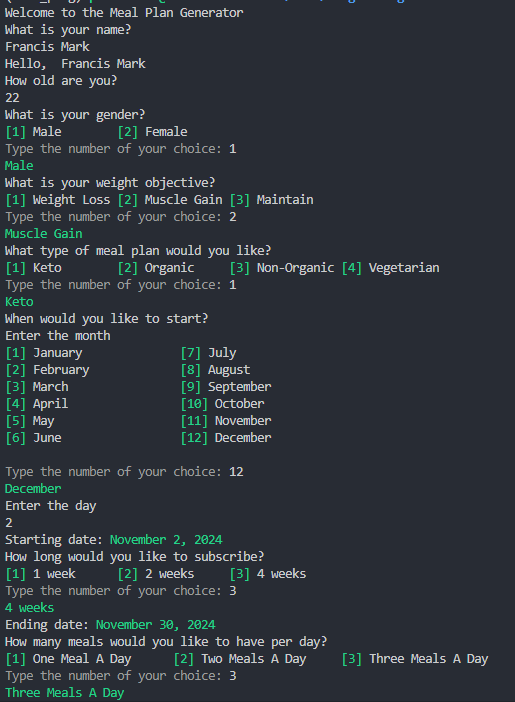
\includegraphics[width=0.65\textwidth]{docs/image.png}
    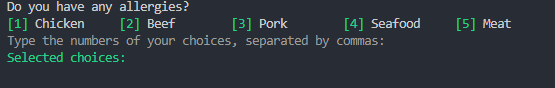
\includegraphics[width=0.65\textwidth]{docs/image-1.png}
    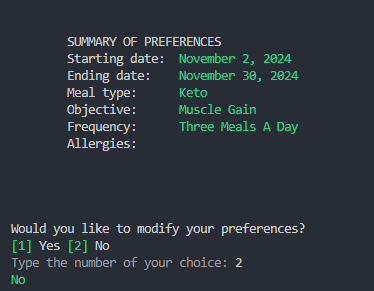
\includegraphics[width=0.65\textwidth]{docs/image-2.png}
    \caption{Sample CMD Output asking the user to input his meal preferences.}
  \end{center}
\end{figure}

\subsection{Meal Plan Output (CMD)}
\begin{figure}[!hbt]
  \begin{center}
    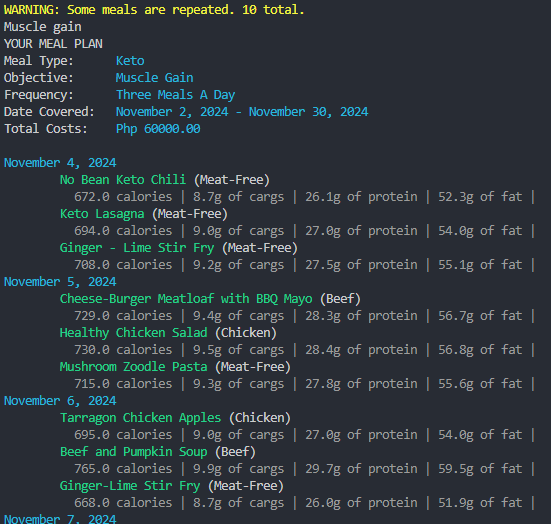
\includegraphics[width=0.65\textwidth]{docs/image-3.png}
    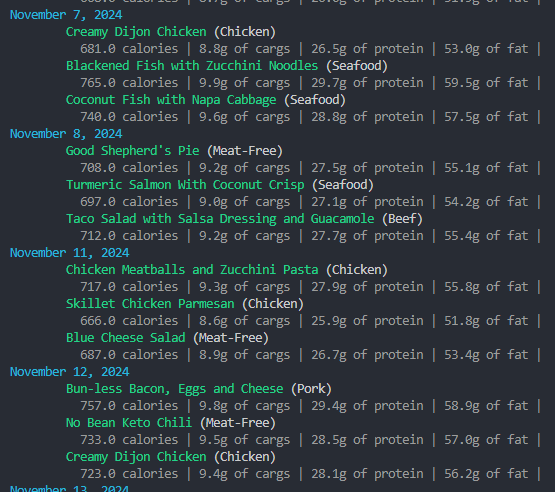
\includegraphics[width=0.65\textwidth]{docs/image-4.png}
    \caption{Sample CMD Output of the Meal Plan.}
  \end{center}
\end{figure}

\subsection{Meal Plan Output (Document)}
\begin{figure}[!hbt]
  \begin{center}
    \fbox{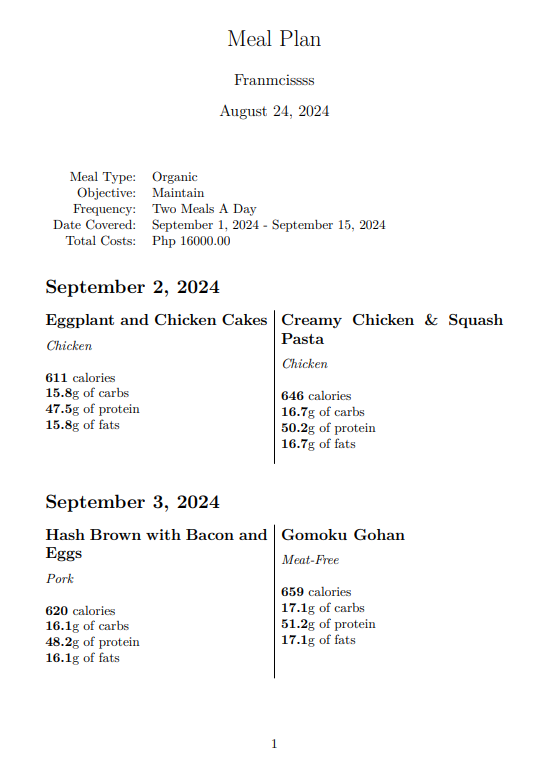
\includegraphics[width=\textwidth]{docs/sample_doc_output.png}}
    \caption{Sample Document Output of the Meal Plan.  Only the first page is shown for demonstration purposes.}
  \end{center}
\end{figure}
\end{document}